
%(BEGIN_QUESTION)
% Copyright 2011, Tony R. Kuphaldt, released under the Creative Commons Attribution License (v 1.0)
% This means you may do almost anything with this work of mine, so long as you give me proper credit

{\it Electrolytic cells} are used in a variety of process industries (aluminum smelting, electroplating, chlorine production) to drive certain endothermic (energy-absorbing) chemical reactions.  The basic concept is to pass large amounts of direct current (DC) through liquid electrolyte solutions, where the electricity will force the desired chemical reaction to take place.

In this system, six electrolytic cells are connected in series, the amount of current through them regulated by a control system.  The ``final control element'' in this electrical system is a device known as a {\it saturable reactor}: an electrical component constructed much like a transformer, designed to impose different amounts of inductive reactance ($X_L$) in an AC circuit with varying amounts of DC control current injected through a ``control winding.''  The greater the DC control current through the control winding, the less inductive reactance in the AC circuit (and therefore more current in the AC circuit).  In this system, a solid-state SCR drive outputs the necessary DC control current to the saturable reactor, at the command of a 4-20 mA signal from the current indicating controller (IIC):

$$\includegraphics[width=15.5cm]{i02510x01.eps}$$

Unfortunately, this control system seems to have a problem.  The indicating recorder (IIR) in the main control room where you are at shows the cells' current to be unstable, slowly varying up and down over time with no predictable pattern.  You are called to investigate the problem, and your first diagnostic test is to have a field operator place the controller (IIC) into {\it manual} mode.

\filbreak

After doing this, you notice that the recorded current is still erratic, showing no sign of stabilizing.

\vskip 10pt

Identify the likelihood of each specified fault for this control system.  Consider each fault one at a time (i.e. no coincidental faults), determining whether or not each fault could independently account for {\it all} measurements and symptoms in this system.

% No blank lines allowed between lines of an \halign structure!
% I use comments (%) instead, so that TeX doesn't choke.

$$\vbox{\offinterlineskip
\halign{\strut
\vrule \quad\hfil # \ \hfil & 
\vrule \quad\hfil # \ \hfil & 
\vrule \quad\hfil # \ \hfil \vrule \cr
\noalign{\hrule}
%
% First row
{\bf Fault} & {\bf Possible} & {\bf Impossible} \cr
%
\noalign{\hrule}
%
% Another row
Poor controller tuning &  &  \cr
%
\noalign{\hrule}
%
% Another row
Rectifying diode failed open &  &  \cr
%
\noalign{\hrule}
%
% Another row
Rectifying diode failed shorted &  &  \cr
%
\noalign{\hrule}
%
% Another row
SCR drive output unstable &  &  \cr
%
\noalign{\hrule}
%
% Another row
Chemical problems in one or more cells &  &  \cr
%
\noalign{\hrule}
%
% Another row
High-resistance earth ground connection &  &  \cr
%
\noalign{\hrule}
%
% Another row
IT-1 faulty &  &  \cr
%
\noalign{\hrule}
%
% Another row
IT-2 faulty &  &  \cr
%
\noalign{\hrule}
} % End of \halign 
}$$ % End of \vbox

\vskip 10pt

Also, trace the direction of electric current through all the cells as well as the voltage drop polarity across each.

\vskip 20pt \vbox{\hrule \hbox{\strut \vrule{} {\bf Suggestions for Socratic discussion} \vrule} \hrule}

\begin{itemize}
\item{} What kinds of current sensors are used in this control system to monitor electrolytic cell current?  Why are two different sensor types used?
\item{} Should there normally be any electrical current flowing into or out of the earth ground at the mid-point of the series cell circuit?  Explain why or why not.
\end{itemize}

\underbar{file i02510}
%(END_QUESTION)





%(BEGIN_ANSWER)

Electrical current direction (conventional flow notation) and voltage polarities:

$$\includegraphics[width=15.5cm]{i02510x02.eps}$$

% No blank lines allowed between lines of an \halign structure!
% I use comments (%) instead, so that TeX doesn't choke.

$$\vbox{\offinterlineskip
\halign{\strut
\vrule \quad\hfil # \ \hfil & 
\vrule \quad\hfil # \ \hfil & 
\vrule \quad\hfil # \ \hfil \vrule \cr
\noalign{\hrule}
%
% First row
{\bf Fault} & {\bf Possible} & {\bf Impossible} \cr
%
\noalign{\hrule}
%
% Another row
Poor controller tuning & $\surd$ &  \cr
%
\noalign{\hrule}
%
% Another row
Rectifying diode failed open &  & $\surd$ \cr
%
\noalign{\hrule}
%
% Another row
Rectifying diode failed shorted &  & $\surd$ \cr
%
\noalign{\hrule}
%
% Another row
SCR drive output unstable & $\surd$ &  \cr
%
\noalign{\hrule}
%
% Another row
Chemical problems in one or more cells & $\surd$ &  \cr
%
\noalign{\hrule}
%
% Another row
High-resistance earth ground connection &  & $\surd$ \cr
%
\noalign{\hrule}
%
% Another row
IT-1 faulty & $\surd$ &  \cr
%
\noalign{\hrule}
%
% Another row
IT-2 faulty &  & $\surd$ \cr
%
\noalign{\hrule}
} % End of \halign 
}$$ % End of \vbox

In this particular scenario, controller tuning would have to be ``poor'' in such a way that it takes insufficient action to regulate normal variations in cell current.  In other words, an {\it under-tuned} controller is possible because it would behave much the same as a controller placed in manual mode, given the assumption that cell current typically varies in the system.

Variations in cell current may be caused by gas bubbles accumulating and then dissipating at the cell electrodes, effectively varying each cell's resistance randomly over time.

%(END_ANSWER)





%(BEGIN_NOTES)


%INDEX% Basics, control loop troubleshooting: determining cause of control problem
%INDEX% Electronics review, saturable reactor
%INDEX% Process: electrolytic chemical cells
%INDEX% Troubleshooting review: electric circuits

%(END_NOTES)


